
\section*{Riti di conclusione}

	\begin{dialoghi}
		\item[\sacerdote] Il Signore sia con voi
		\item[\assemblea] E con il tuo spirito.
		\item[\sacerdote] Dio, eterno Padre, vi conservi uniti nel reciproco amore; la pace di Cristo abiti in voi e rimanga sempre nella vostra casa.
		\item[\assemblea] Amen
		\item[\sacerdote] Abbiate benedizione nei figli, conforto dagli amici, vera pace con tutti.
		\item[\assemblea] Amen
		\item[\sacerdote] Siate nel mondo testimoni dell'amore di Dio, perché i poveri e i sofferenti, che hanno sperimentato la vostra carità, vi accolgano grati un giorno nella casa del Padre.
		\item[\assemblea] Amen
		\item[\sacerdote] E su voi tutti che avete partecipato a questa liturgia nuziale, scenda la benedizione di Dio onnipotente, Padre e Figlio (+) e Spirito Santo.
		\item[\assemblea] Amen
		\item[\sacerdote] Nella Chiesa e nel mondo siate testimoni del dono della vita e dell'amore che avete celebrato. Andate in pace
		\item[\assemblea] Rendiamo grazie a Dio
	\end{dialoghi}


\subsection*{Canto finale: \textit{Resta accanto a me}}

	\begin{mystrofe}
		\ritornello{Ora vado sulla mia strada \\
		con l'amore tuo che mi guida \\
		o Signore, ovunque io vada \\
		resta accanto a me. \\}
	\end{mystrofe}

	\begin{mystrofe}
		Io ti prego, stammi vicino \\
		ogni passo del mio cammino \\
		ogni notte, ogni mattino \\
		resta accanto a me. \\
	\end{mystrofe}

	\begin{mystrofe}
		Il tuo sguardo puro sia luce per me \\
		e la tua parola sia voce per me. \\
		Che io trovi il senso del mio andare \\
		solo in te, \\
		nel tuo fedele amare il mio perché. \\
	\end{mystrofe}

	\begin{mystrofe}
		\ritornello{}
	\end{mystrofe}

	\begin{mystrofe}
		Fa' che chi mi guarda non veda che te \\
		fa' che chi mi ascolta non senta che te \\
		e chi pensa a me, fa' che nel cuore \\
		pensi a te e trovi quell'amore \\
		che hai dato a me. \\
	\end{mystrofe}

	\begin{mystrofe}
		\ritornello{}
	\end{mystrofe}

\vfill
\begin{center}
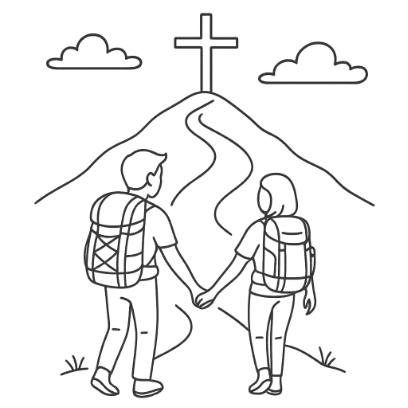
\includegraphics[width=\textwidth]{src/assets/img/fine.png}
\end{center}
\vfill